\documentclass{beamer}
\beamertemplatenavigationsymbolsempty
\usecolortheme{beaver}
\setbeamertemplate{blocks}[rounded=true, shadow=true]
\setbeamertemplate{footline}[page number]
%
\usepackage[utf8]{inputenc}
\usepackage[english,russian]{babel}
\usepackage{amssymb,amsfonts,amsmath,mathtext}
\usepackage[]{algorithmic}
\usepackage{subfig}
\usepackage[all]{xy} % xy package for diagrams
\usepackage{array}
\usepackage{tikz}
\usepackage{multicol}% many columns in slide
\usepackage{hyperref}% urls
\usepackage{hhline}%tables
% Your figures are here:
\graphicspath{ {fig/} {../fig/} }

%----------------------------------------------------------------------------------------------------------
\title[\hbox to 56mm{Петли скрытой обратной связи}]{ Условия существования петель скрытой \\ обратной связи в рекомендательных системах }
\author[А.\,А. Пилькевич]{Антон Александрович Пилькевич}
\institute{Московский физико-технический институт}
\date{\footnotesize
\par\smallskip\emph{Курс:} Автоматизация научных исследований\par (практика, В.\,В.~Стрижов)/Группа 813
\par\smallskip\emph{Эксперт:} А.\,С.~Хританков
\par\smallskip\emph{Консультант:} А.\,С.~Хританков
\par\bigskip\small 2021}
%----------------------------------------------------------------------------------------------------------
\begin{document}
%----------------------------------------------------------------------------------------------------------
\begin{frame}
\thispagestyle{empty}
\maketitle
\end{frame}
%-----------------------------------------------------------------------------------------------------
\begin{frame}{Цель исследования}
\begin{block}{Цель}
  Исследование условий существования петель обратной
связи в рекоммендательной системе с алгоритмом Thompson Sampling в условиях зашумлённости выбора пользователя.
\end{block}
\begin{block}{Задача}
  Нахождение математического описания условий возникновения петель и экспериментальная их проверка. 
\end{block}
\begin{block}{Решение}
  Усреденение смещение интереса и анализ зависимости от параметров шума. 
  Моделирование рекомендательной системы и поведения пользователя.
\end{block}
\end{frame}
%-----------------------------------------------------------------------------------------------------
\begin{frame}{Петли в рекомендательных системах}

\begin{columns}[c]
\column{0.5\textwidth}
Отклик $c_t^i$ для рекомендации $\mathbf{a_t}$:
\begin{gather*}
    c_t^i \sim \text{Bern} \left(\sigma\left(\mu_t^i (a_t^i) + \mathbin{\color{red} q_t^i } \right) \right). 
\end{gather*}
Интерес $\mu_t^i$:
\begin{gather*}
    \mu_{t+1} - \mu_{t} = \delta_t c_t - \delta_t (1 - c_t),\\ 
\end{gather*}

Определение петель: 
\begin{gather*}
  \color{red} \lim_{t \to \infty} \|\mu_t - \mu_0 \|_2 = \infty.
\end{gather*}
\column{0.6\textwidth}
\begin{tikzpicture}[
  node distance={13mm}, thick, 
  roundnode/.style={circle, draw=blue!60, fill=blue!5, very thick, minimum size=4mm},
  squarednode/.style={rectangle, draw=red!60, fill=red!5, very thick, minimum size=4mm},
] 
\node[roundnode] (1) {$a^1$}; 
\node[roundnode] (2) [right of=1] {$a^2$};
\node[roundnode] (3) [right of=2] {$a^3$};
\node[squarednode] (5) [below of=1]{$\mu^1$}; 
\node[squarednode] (6) [below of=2] {$\mu^2$};
\node[squarednode] (7) [below of=3] {$\mu^3$};
\node[draw] (4) [below of=6] {$User$};

\draw[-] (4) -- (5);
\draw[-] (4) -- (6);
\draw[-] (4) -- (7);

\draw[blue,->] (5) to [out=150, in=-150, looseness=1.] node[left]{$c^1 = 1$} (1);
\draw[blue,->] (6) to [out=150, in=-150, looseness=1.]  (2);
\draw[blue,dotted] (7)  to [out=150, in=-150, looseness=1.] node[right]{$c^3 = 0$} (3);

\draw[red,->] (1) to [out=-30, in=30, looseness=1.] node[left]{$+\delta^1$}(5);
\draw[red,->] (2) to  [out=-30, in=30, looseness=1.] (6);
\draw[red,->] (3) to  [out=-30, in=30, looseness=1.]node[right]{$-\delta^3$}(7);
\end{tikzpicture} 
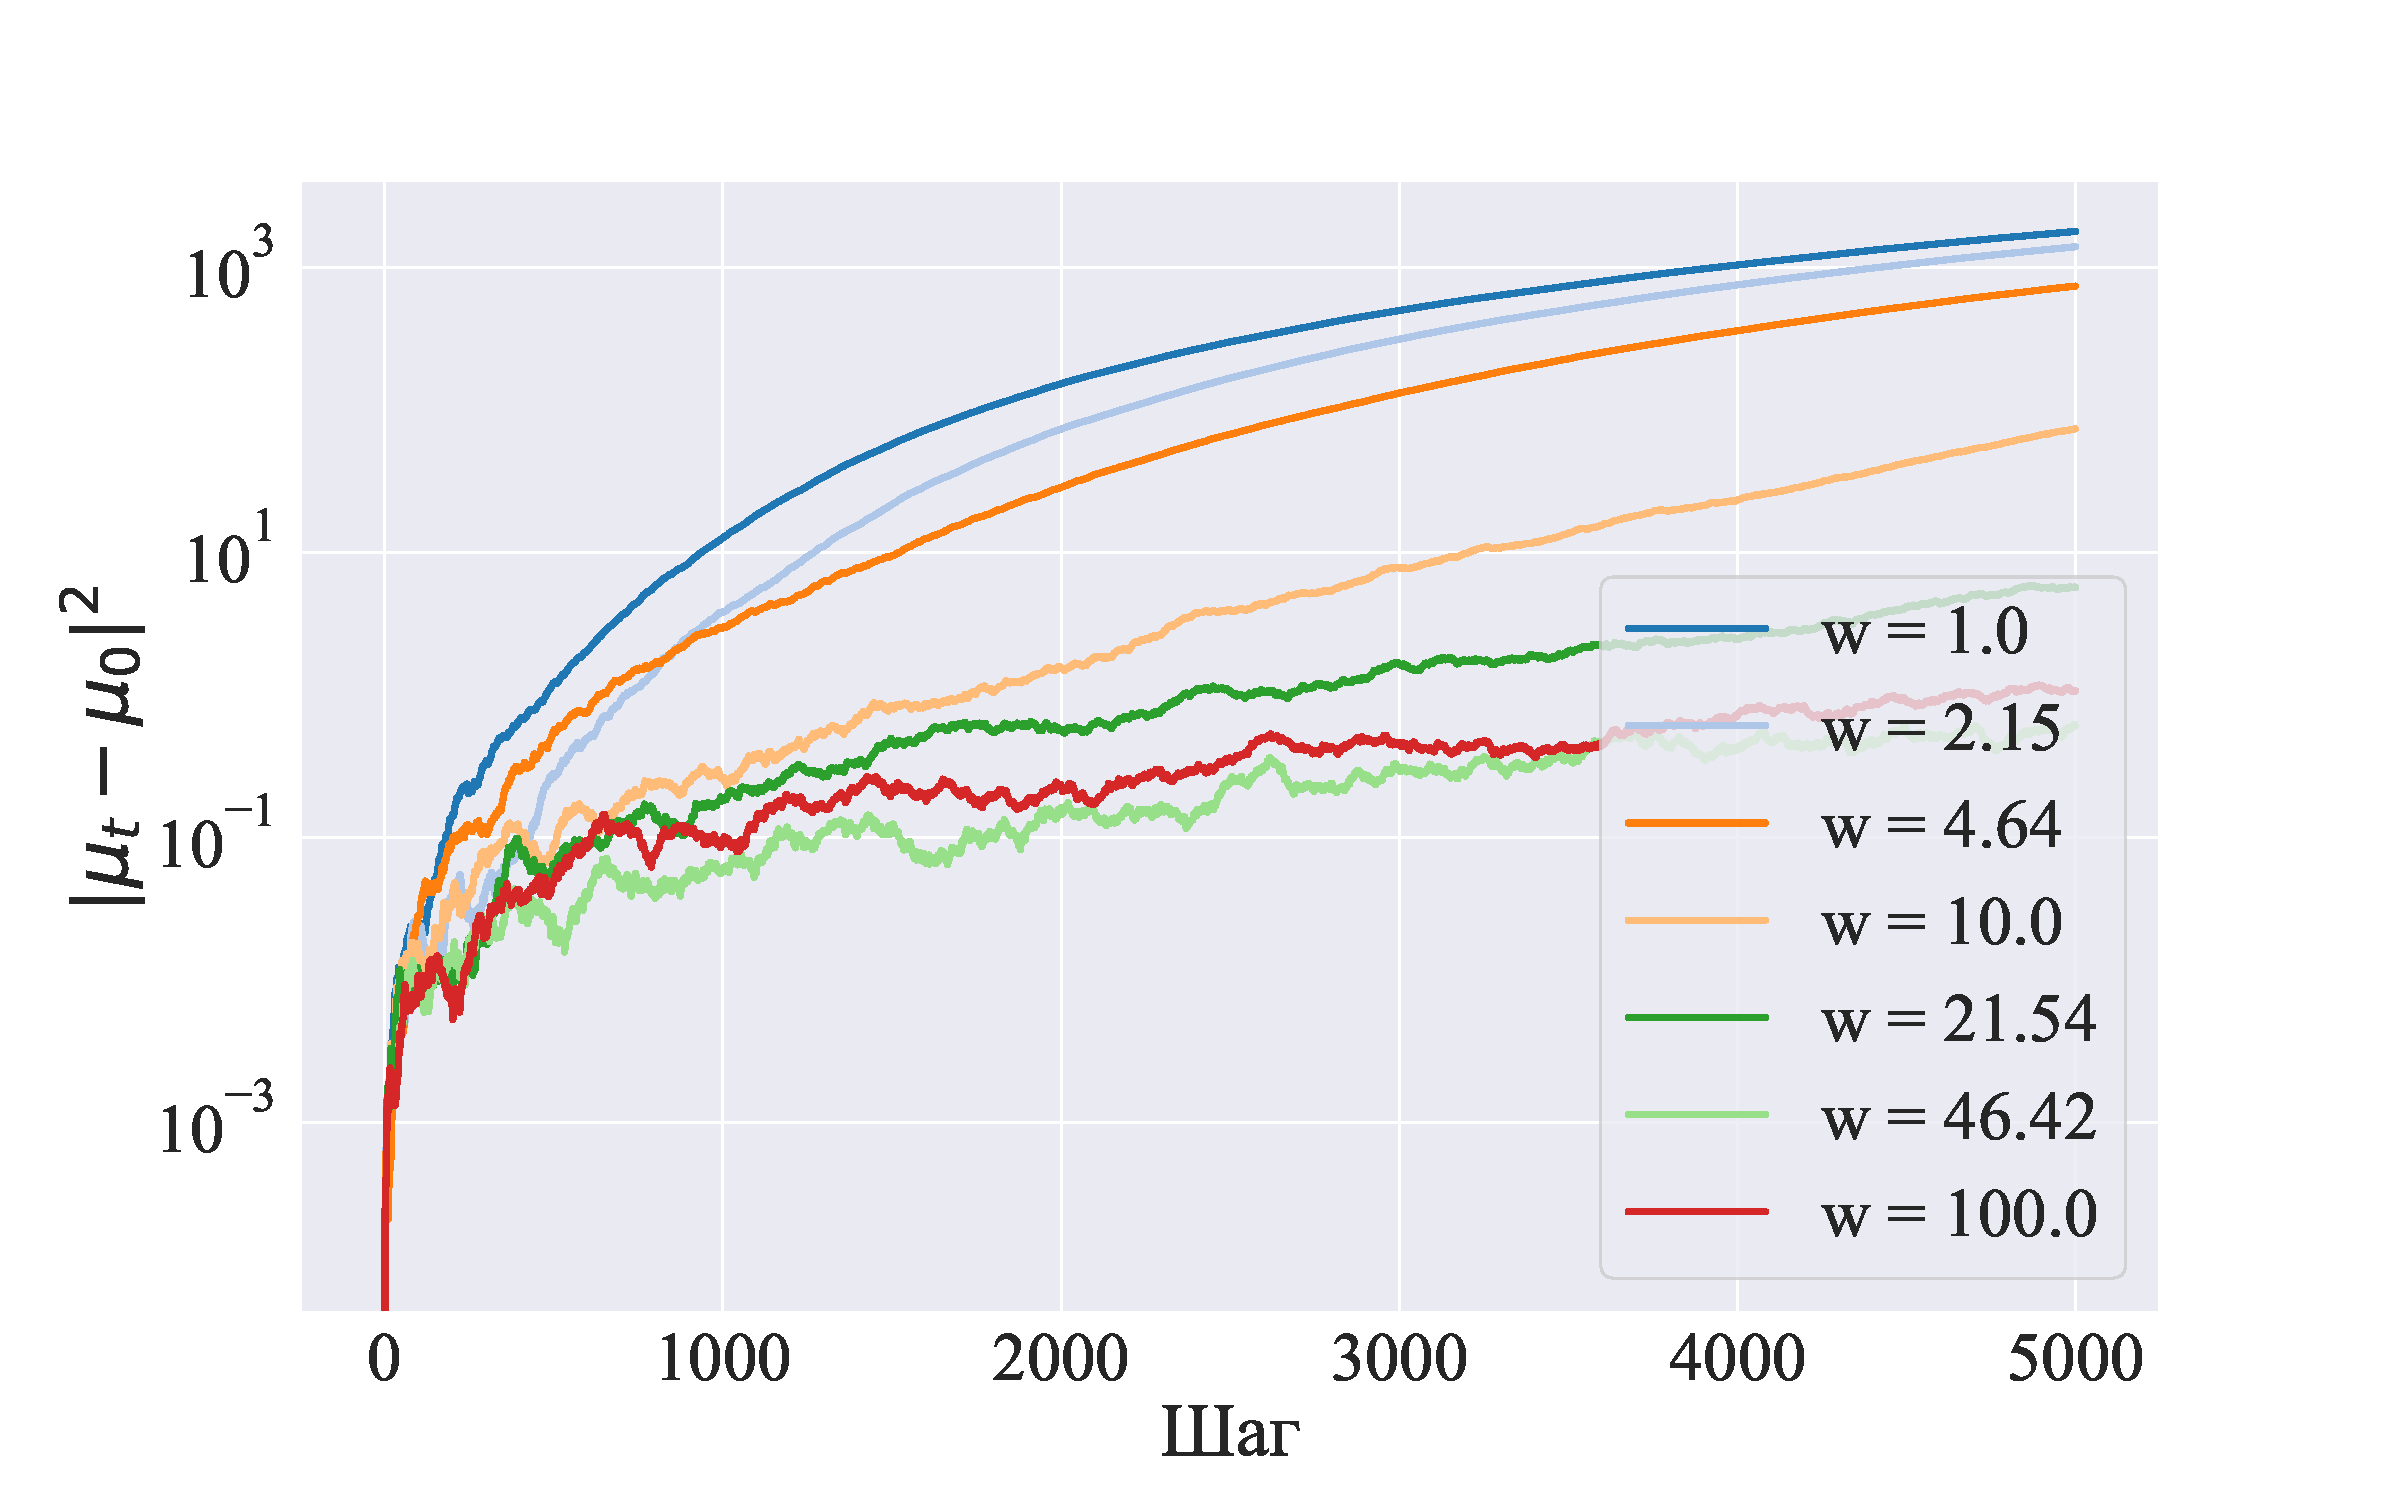
\includegraphics[width=7cm]{../norm_interest.pdf}
\end{columns}
\end{frame}


%----------------------------------------------------------------------------------------------------------
\begin{frame}{Публикации по теме}
\begin{enumerate}
    \item
      \textcolor{black}{Ray~Jiang, Silvia~Chiappa, Tor~Lattimore,Andr{\'a}s Gy{\"o}rgy, Pushmeet~Kohli.}
      \textcolor{blue}{Degenerate Feedback Loops in Recommender Systems}.
    \BibJournal{CoRR}, 2019, Vol. abs/1902.10730,
	  URL: \BibUrl{https://arxiv.org/abs/1902.10730}.

  \item
    \textcolor{black}{Khritankov, Anton.}
    \textcolor{blue}{Hidden Feedback Loops in Machine Learning Systems: A simulation Model and Preliminary Results}//
    \BibJournal{Springer}, 2021, P.~54--65.

  \item
    \textcolor{black}{Daniel Russo, Benjamin Van Roy, Abbas Kazerouni, Ian Osband.}
    \textcolor{blue}{A Tutorial on Thompson Sampling}//
    \BibJournal{CoRR}, 2017, Vol. abs/1707.02038,
	  URL: \BibUrl{https://arxiv.org/abs/1707.02038}.
  \end{enumerate}
\end{frame}
%----------------------------------------------------------------------------------------------------------
\begin{frame}{Модель данных}
  Множество объектов $M$, рекомендации $(a^1, \dots, a^l) \in M$, кол-во выдач $T$.
  Задаётся ф-ия описывающая интерес пользователя  в начальный момент времени $\mu_0 : M \to \mathbb{R}$.

\bigskip

\begin{columns}[T]
\column{0.5\textwidth}
\textcolor{blue}{Аддитивный шум:}   
\begin{gather*}
    c_t^i \sim \text{Bern} \left(\sigma\left(\mu_t^i (a_t^i) + \mathbin{\color{red} q_t^i } \right) \right), \\ 
    q_t^i \sim U[-w, w], \\
\mu_{t+1} - \mu_{t} = \delta_t c_t - \delta_t (1 - c_t), \\
\delta_t \sim U[0, 0.01].
  \end{gather*}

\column{0.5\textwidth}
\textcolor{blue}{Накопительный шум:}   
\begin{gather*}
  c_t^i \sim Bern \left(\sigma(\mu_t(a_t^i)) \right), \\
  \begin{align*}
    \mu_{t+1} - \mu_{t} =~&\delta_t c_t (\mathbin{ \color{red} 1 + b \cdot l_t})~- \\ 
                        &\delta_t (1 - c_t) (\mathbin{ \color{red} 1 + b \cdot s_t}),
\end{align*} \\
  s_t \sim \text{Geom}(1 - \sigma(\mu_t(a_t)), \\
  l_t \sim \text{Geom}(\sigma(\mu_t(a_t)). 
\end{gather*}
\end{columns}
\bigskip
\textcolor{blue}{Определение петли}:
\begin{gather*}
  \color{red} \lim_{t \to \infty} \|\mu_t - \mu_0 \|_2 = \infty.
\end{gather*}
\end{frame}
%----------------------------------------------------------------------------------------------------------
\begin{frame}{Thompson Sampling}
Априорное распределение для параметров интереса: 
\[Beta(1, 1) = U[0, 1].\] 
Апостериорное распределение для элемента $a^i \in M$ описывается $Beta(\alpha_t^i, \beta_t^i)$. 
Параметры обновляются по закону:
\[\alpha_{t+1} = \alpha_t + c_t, \beta_{t+1} = \beta_t + 1 - c_t.\]
Задача оптимизации алгоритма:
\begin{gather*}  
\max_{c_t^i} \sum_{t = 1}^T \sum_{i = 1}^l c_t^i = T \cdot l,\\ 
   T \cdot l - \sum_{t = 1}^T \sum_{i = 1}^l c_t^i \to \min_{b}. 
\end{gather*}
\end{frame}
%----------------------------------------------------------------------------------------------------------
\begin{frame}{Возникновение петли}
Назовём \textit{режимом работы TS с фиксированными лидерами} поведение алгоритма, в котором TS не меняются элементы рекомендаций.
  \begin{block}{Утверждение}
  Пусть  TS работает в режиме c фиксированными лидереми начиная с какого-то момента времени $\tau$ и используется аддитивная модель шума. 
  Для любых $w$:
\begin{gather*}
  \color{red} \lim_{t \to \infty} \|\mu_t - \mu_0 \|_2 = \infty.
\end{gather*}
  \end{block}
  \begin{block}{Анализ результов}
  \begin{itemize}
      \item Любой несмещённый аддитивный шум не влияет на возникновение петли. 
      \item При достаточно большом значение $\mu_t$ из-за $\sigma (x)$ шум $w$ перестаёт сколько-то значимо изменять истинный интерес. 
  \end{itemize}
  \end{block}
\end{frame}
%----------------------------------------------------------------------------------------------------------
\begin{frame}{Вычислительный эксперимент}
\begin{block}{Цель}
Проверка гипотезы о возникновении петель при параметрах шума, найденных из теоретических соотношений. 
\end{block}

\begin{block}{Алгоритм}
\begin{algorithmic}
  \REQUIRE{M, l, T, w, b}
  \STATE Инициализировать начальные значения()
  \FOR{$t$ от $1$ до $T$} 
  \STATE $r_t \leftarrow$ Предсказать рекомендацию()
    \STATE $c_t \leftarrow$ Сгенерировать отклик($r_t$, w, b)
    \STATE Обновить параметры алгоритма($c_t$)
    \STATE Обновить интерес($c_t$)
    \STATE Cохранить текущие значения($t, c_t, \mu_t$)
  \ENDFOR
\end{algorithmic}
\end{block}

\end{frame}
%----------------------------------------------------------------------------------------------------------
\begin{frame}{Аддитивный шум} 
\begin{columns}[T]
\column{0.5\textwidth}
Норма интeреса от итерации.
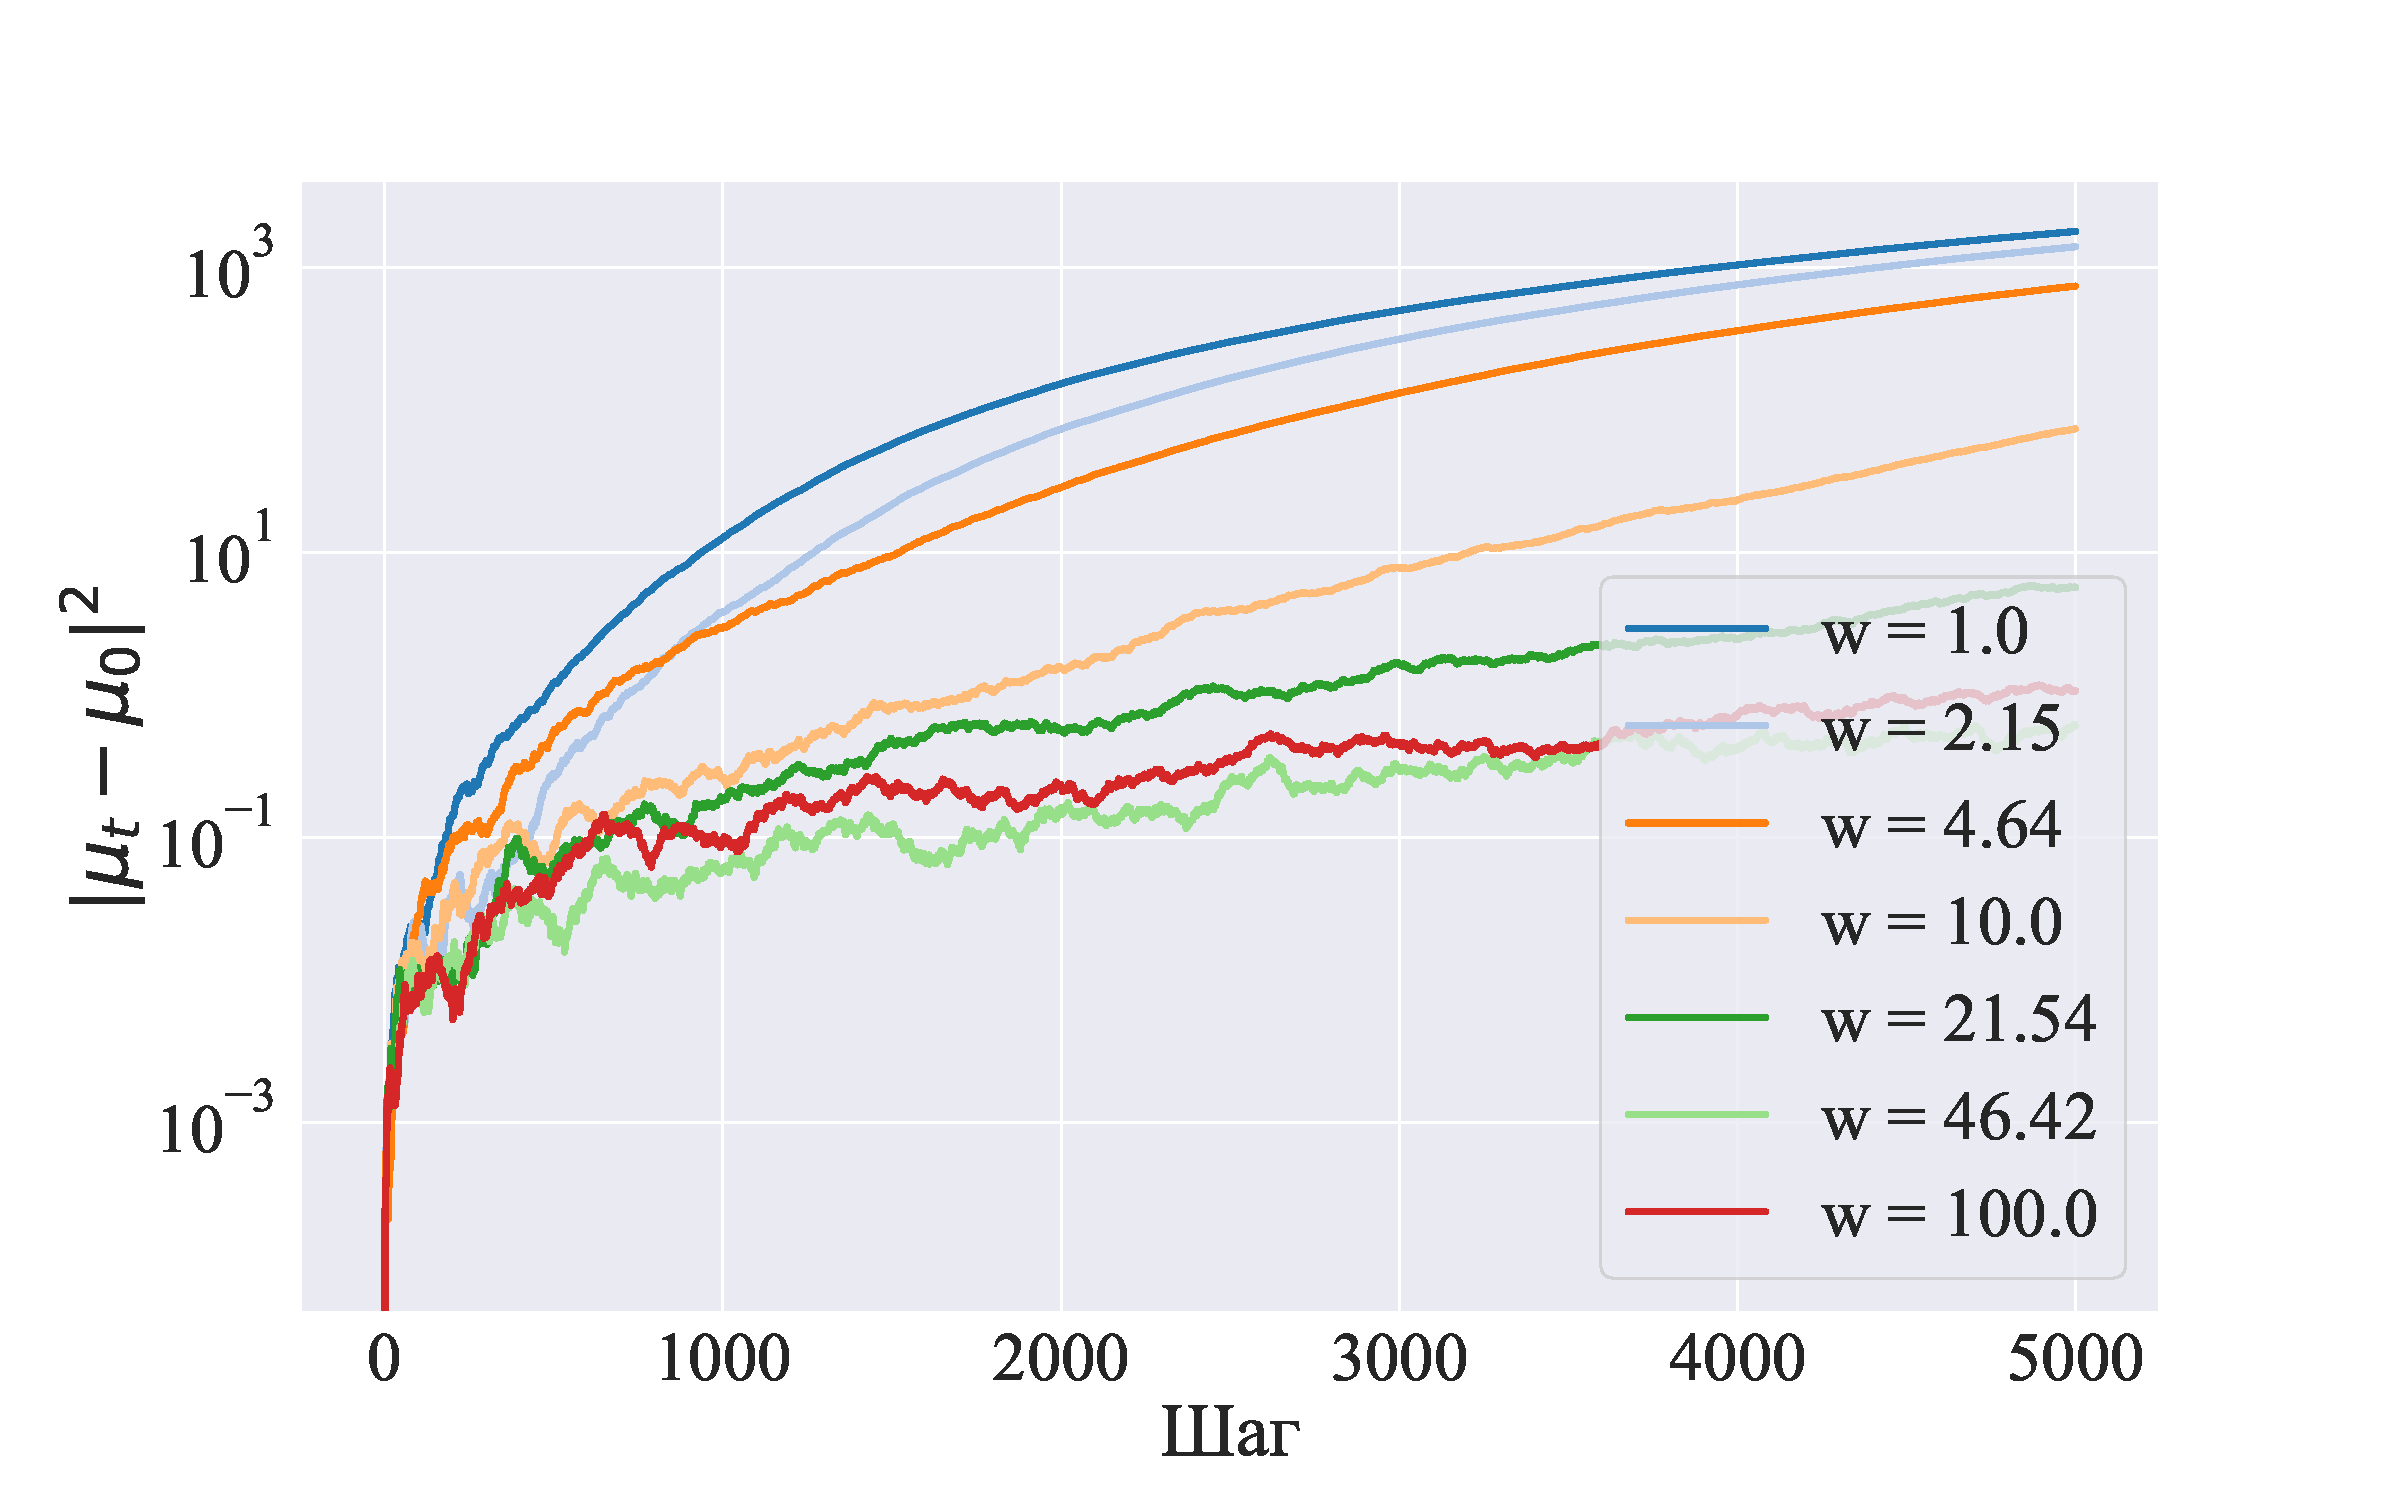
\includegraphics[width=6cm]{../norm_interest.pdf}
\column{0.5\textwidth}
Сумма откликов от итерации.  
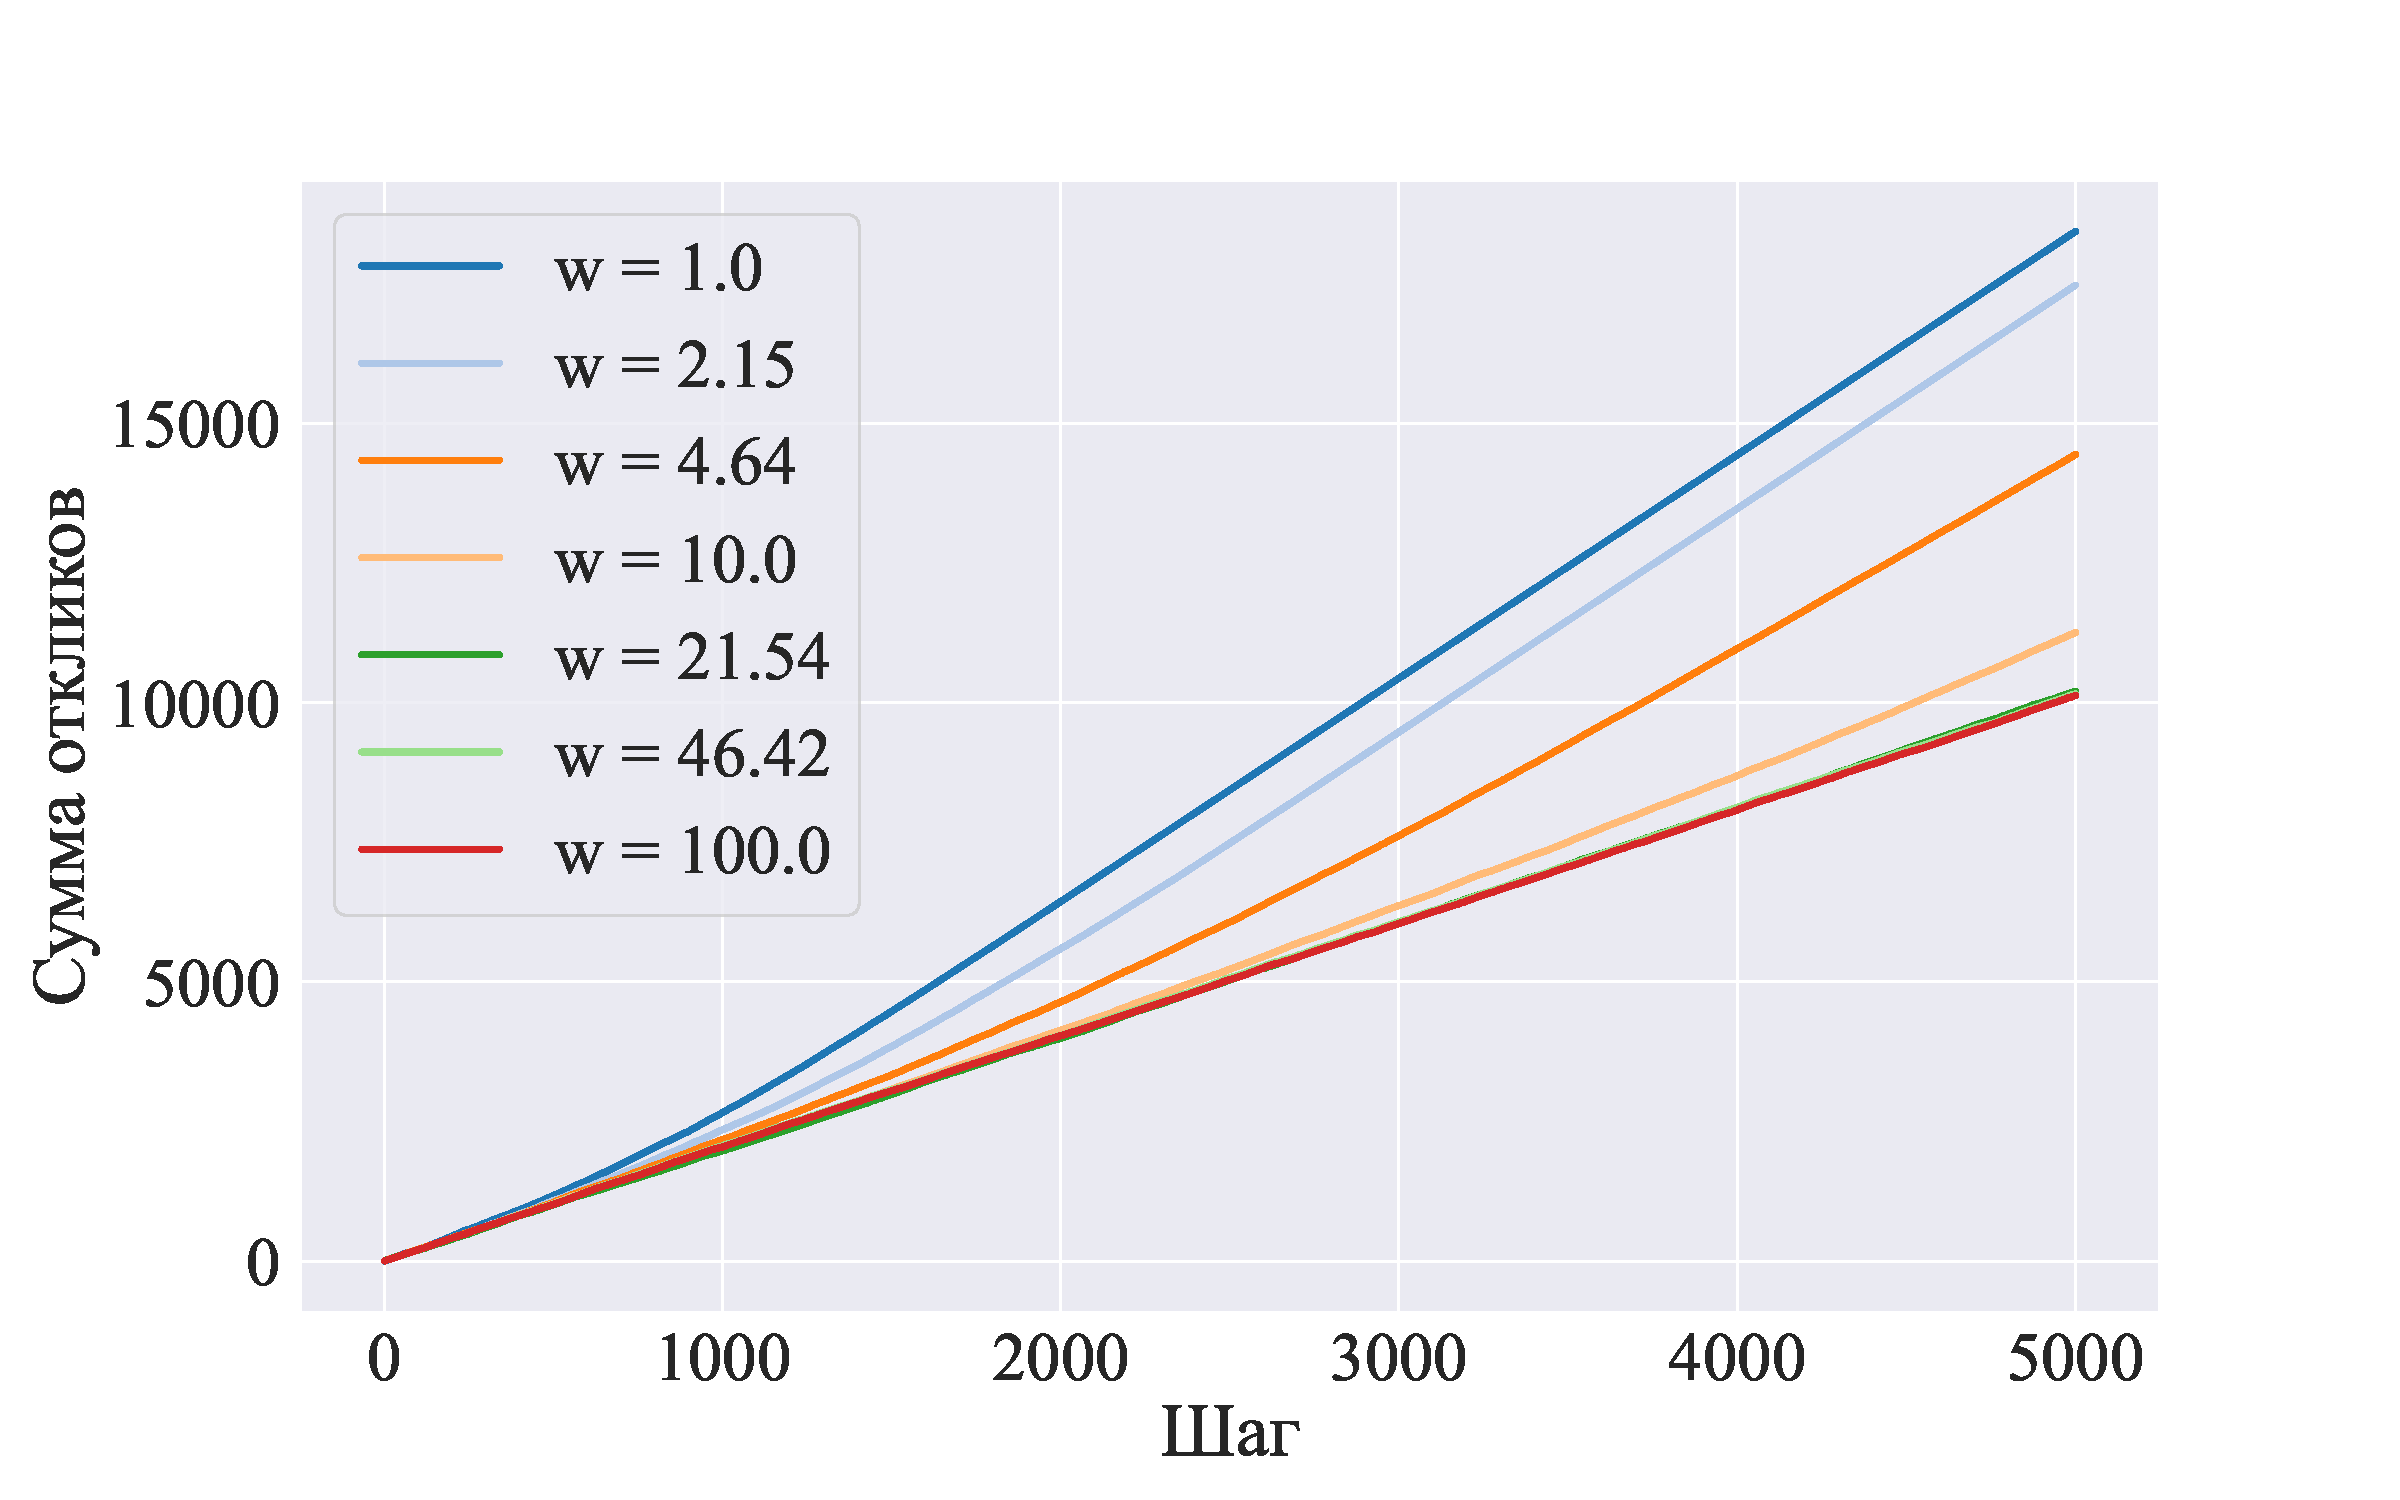
\includegraphics[width=6cm]{../rewards.pdf}
\end{columns}

\end{frame}
%------------------------------------------------------------------------------------
\begin{frame}{Накопительный шум}
\begin{columns}[T]
\column{0.5\textwidth}

Разброс нормы интереса
\begin{center}
  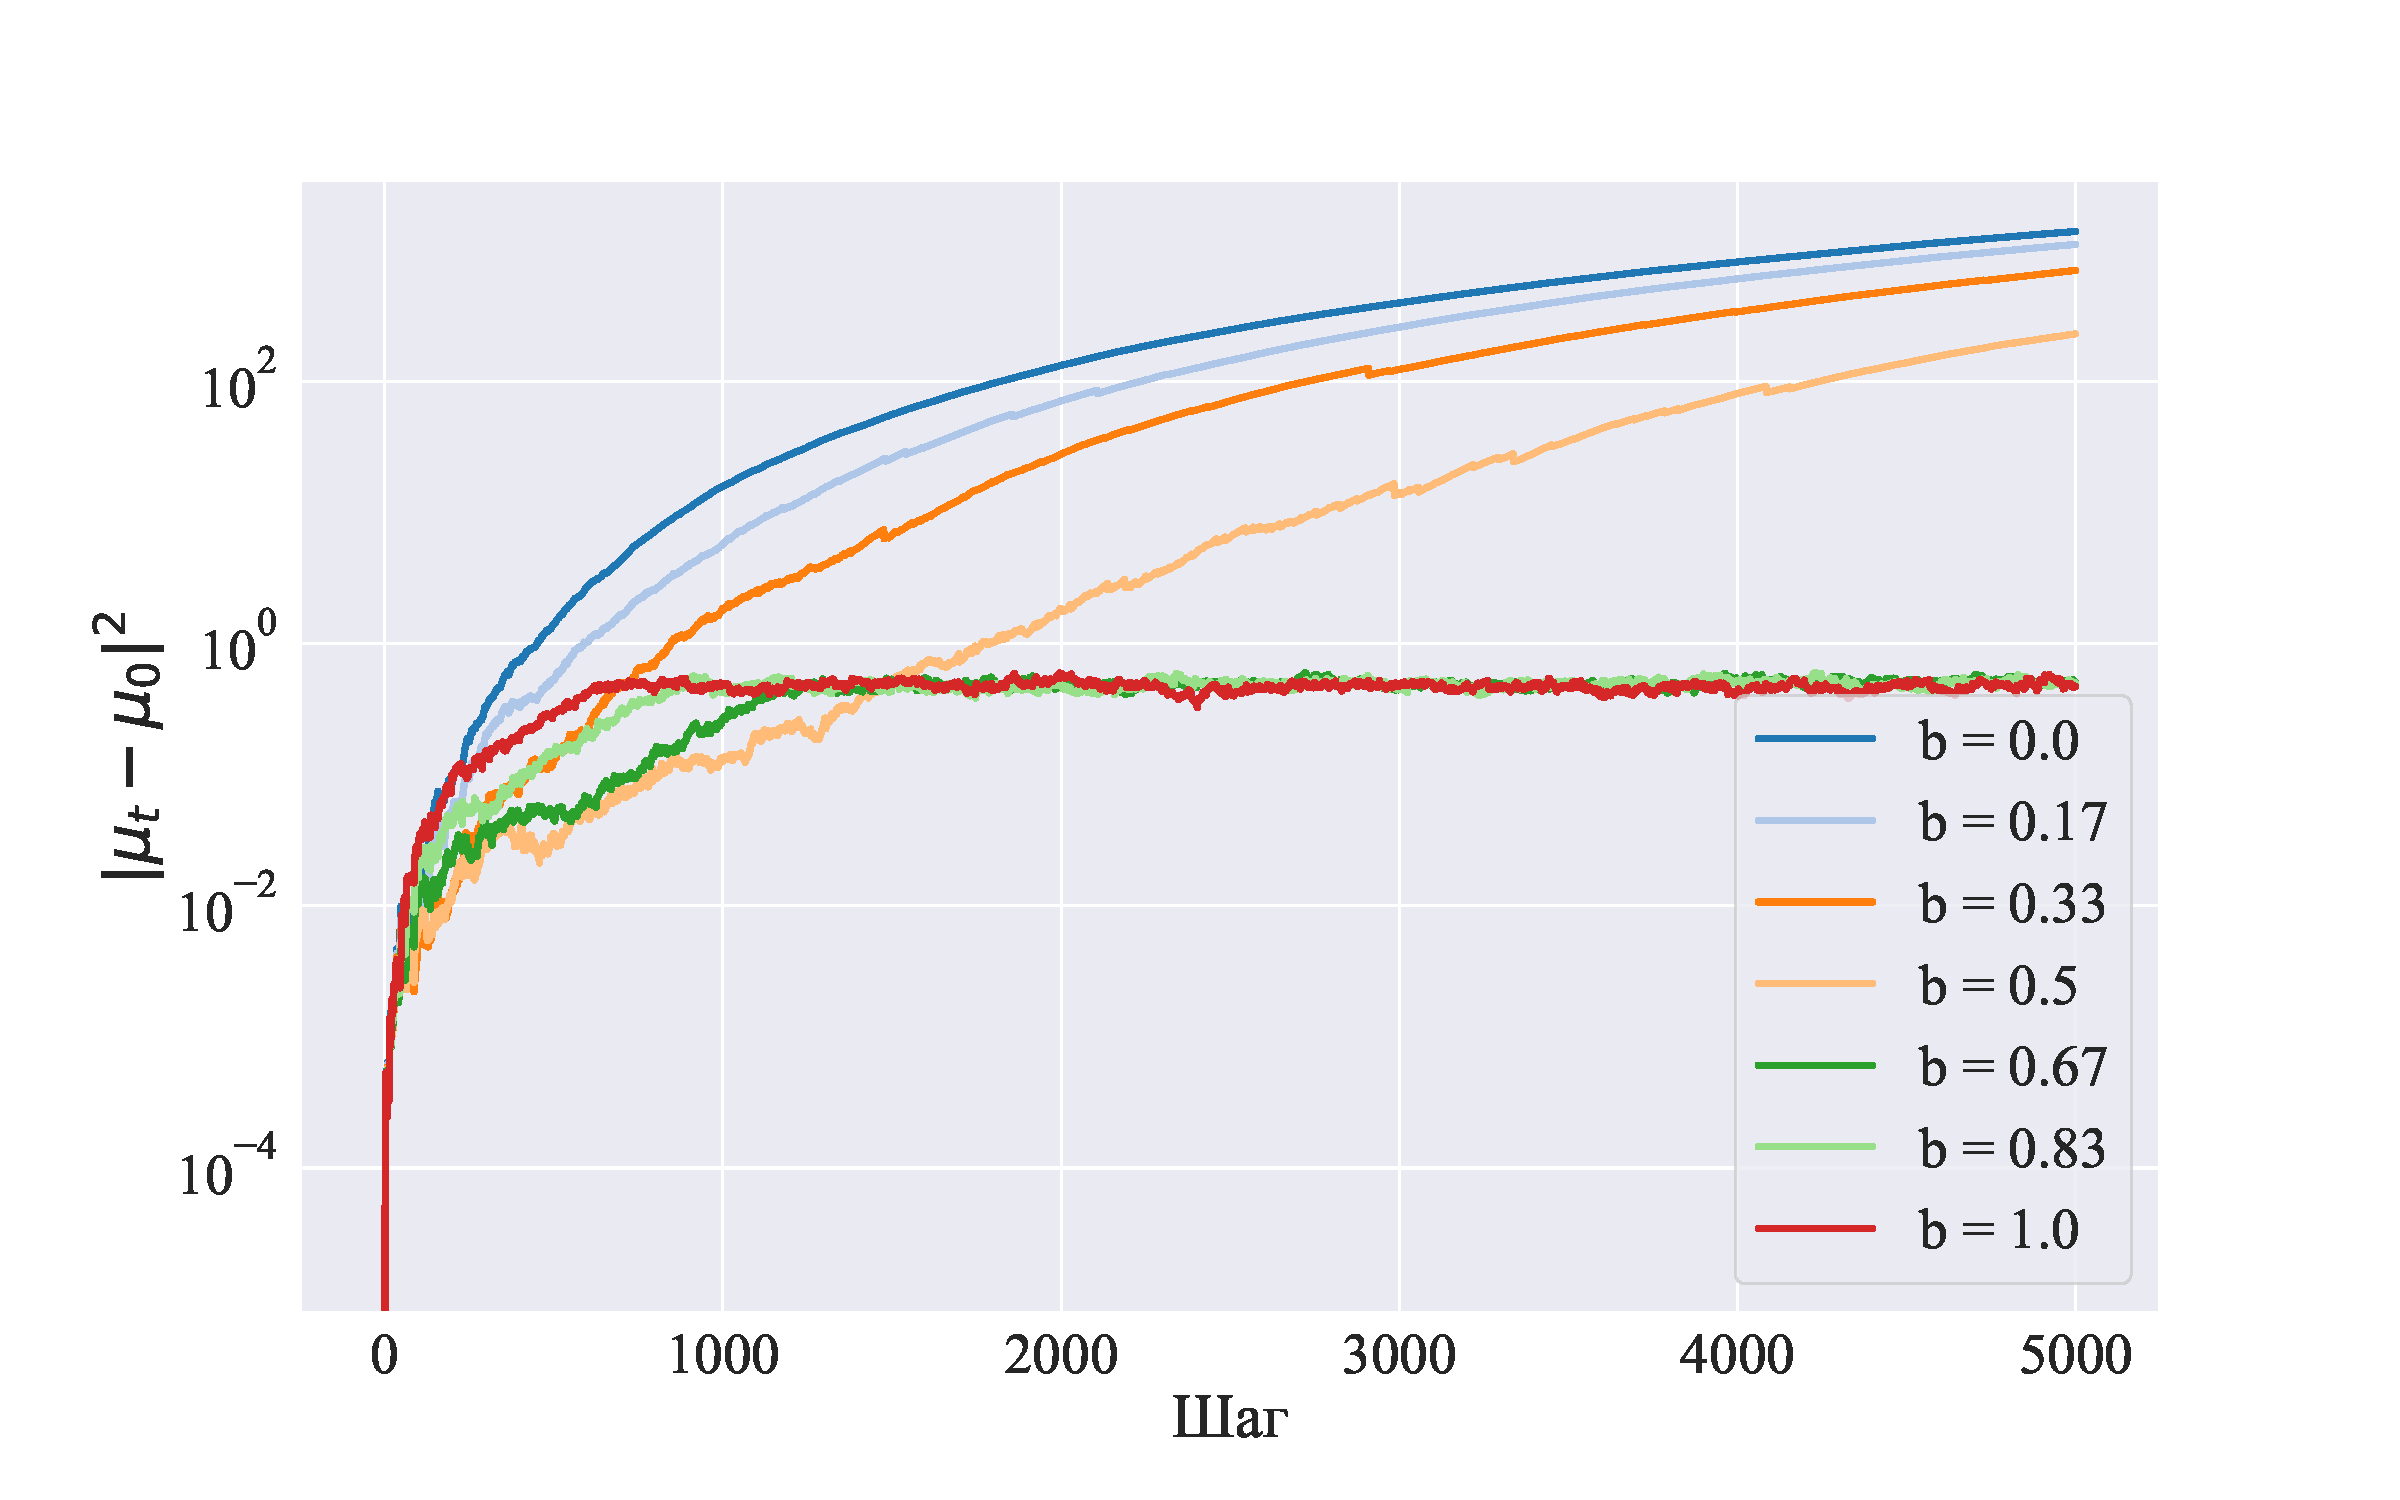
\includegraphics[width=6cm]{../winstreak_norm_interest.pdf}
\end{center}
\column{0.5\textwidth}
Распределение максимума интереса после $2000$ шагов.
\begin{center}
  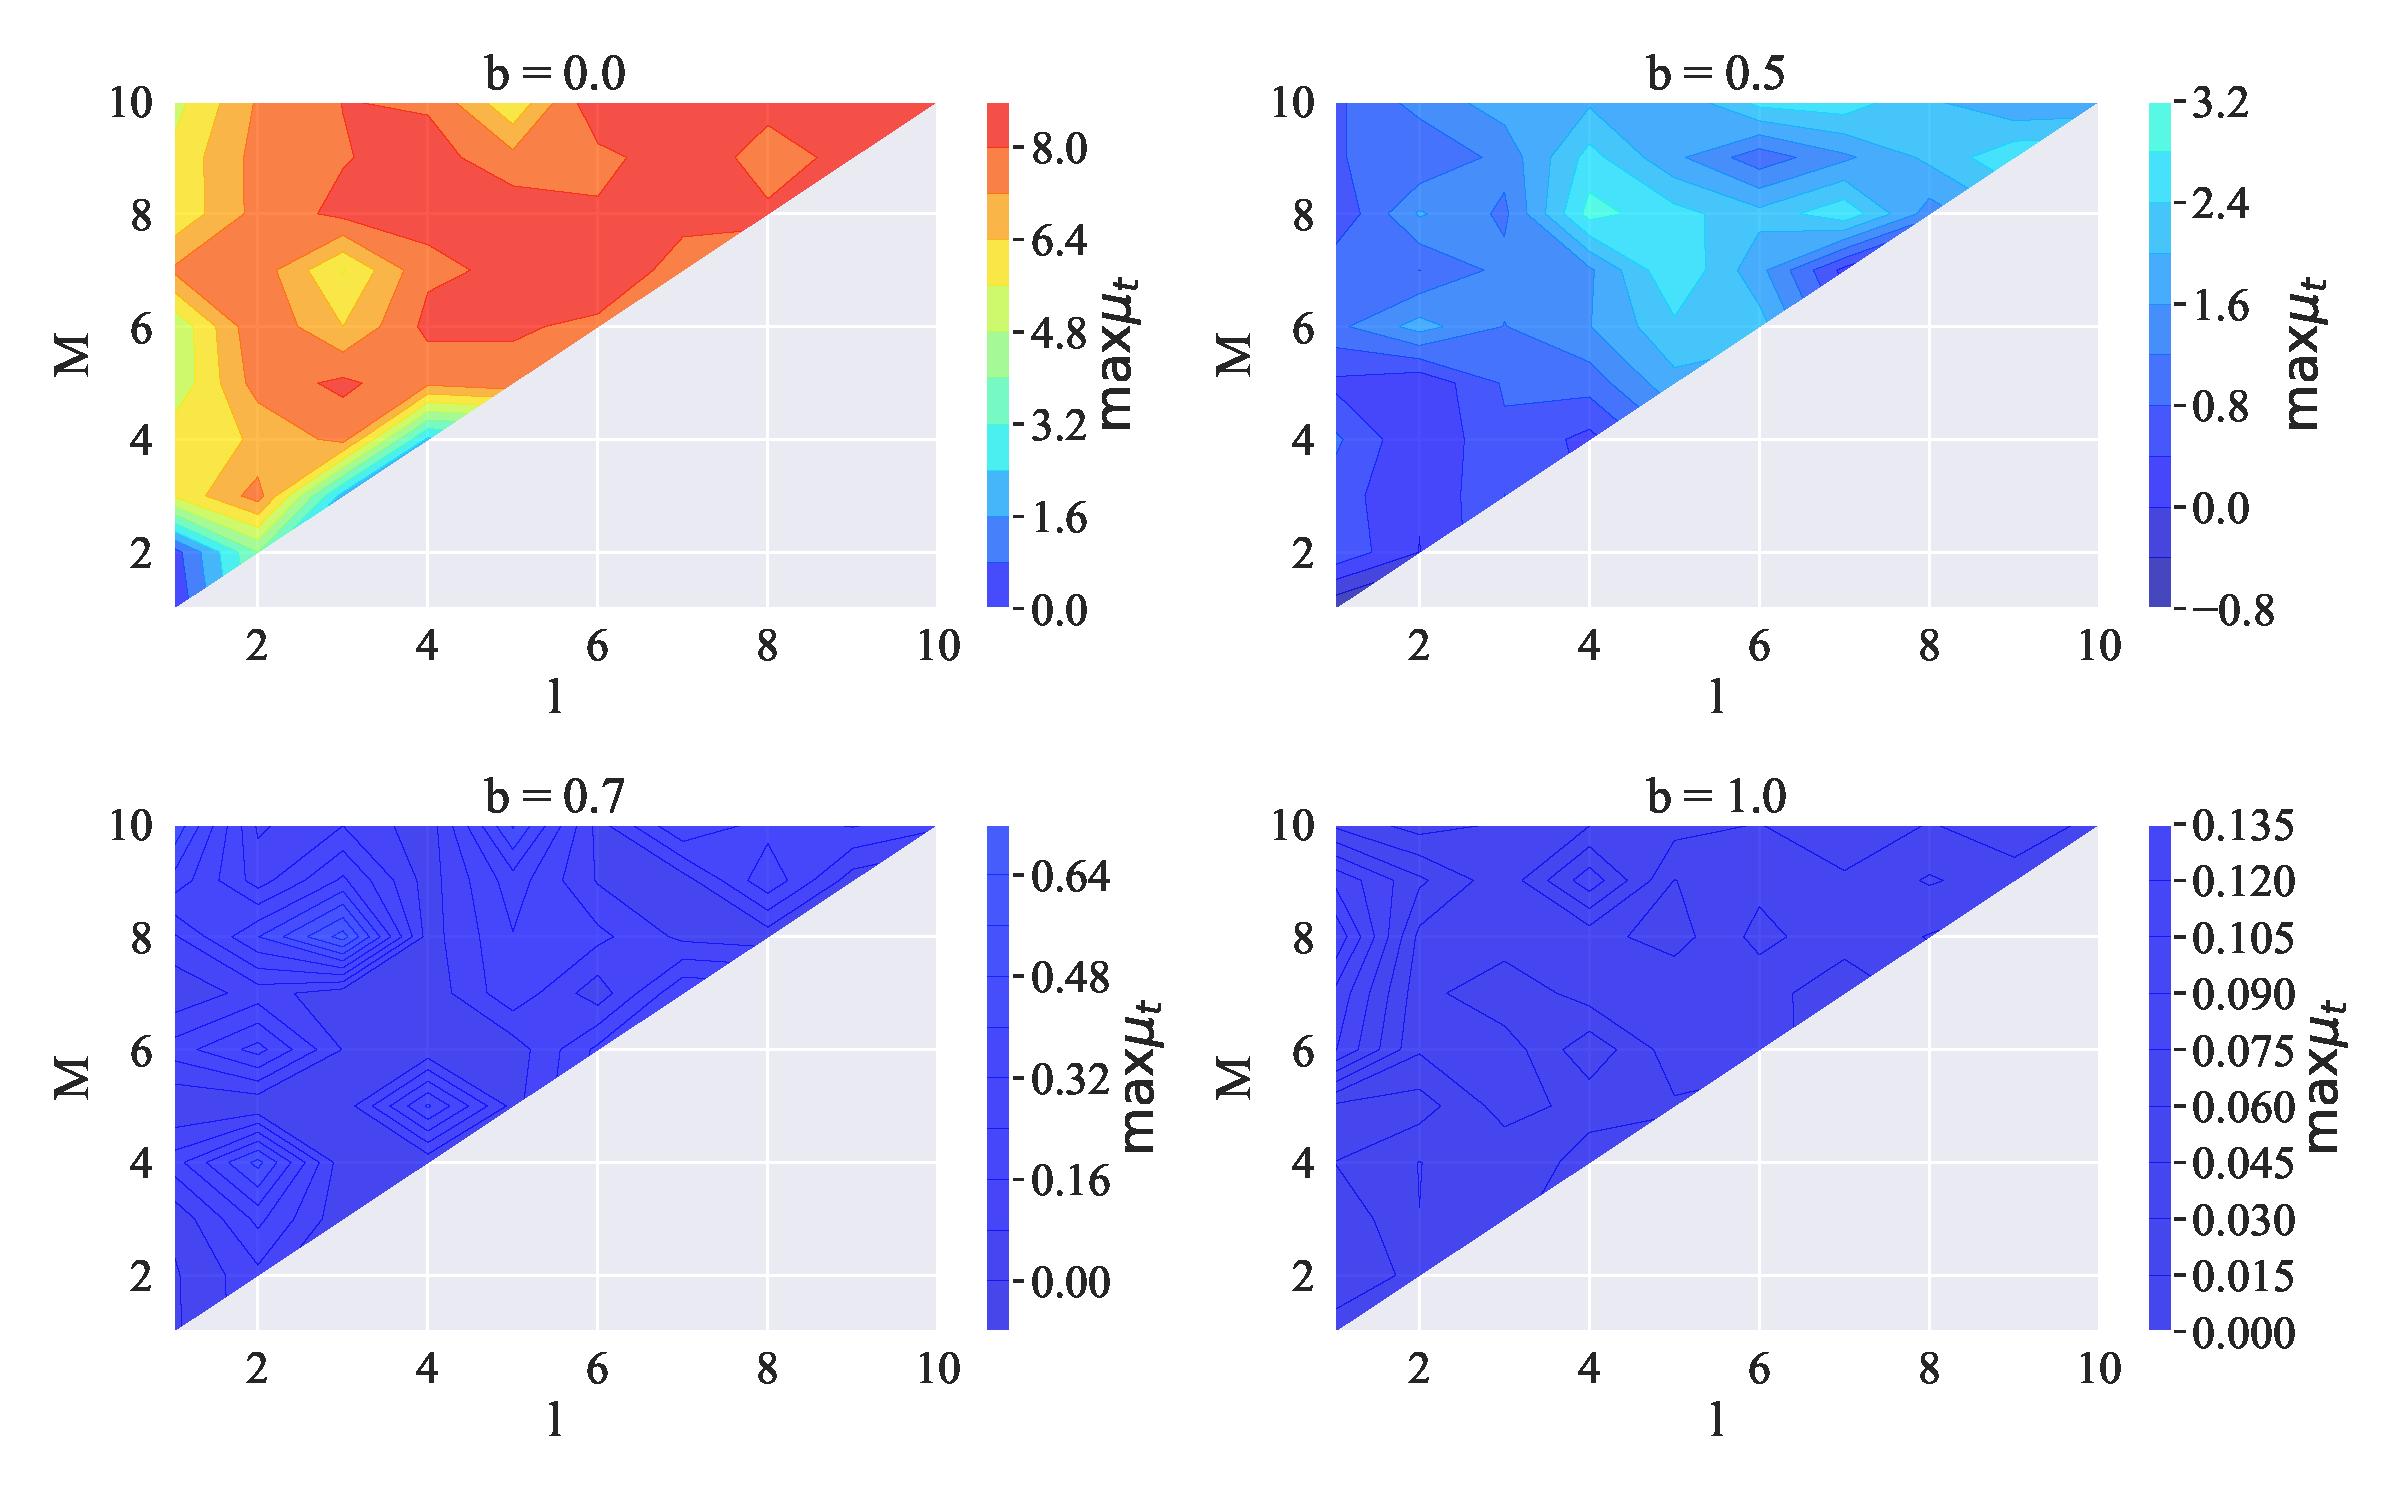
\includegraphics[width=6cm]{../countour_Mlb_part.pdf}
\end{center}
\end{columns}
\end{frame}
%----------------------------------------------------------------------------------------------------------
\begin{frame}{Заключение}
  \begin{itemize}
      \item Поставлена задача с учётом аддитивного шума в ответах пользователя для рекомендательная системы использующей алгоритм TS
      \item Поставлена задача с учётом корреляции между обновлением интереса. 
      \item Получено, что при любых парамeтрах аддитивного шума возникает петля  
      \item Показано, что утверждение подтверждается на эксперименте.
      \item Показано, что при накопительном шуме петли не возникают.
  \end{itemize}
\end{frame}
%----------------------------------------------------------------------------------------------------------
\end{document} 
